% ----------------------------------------------------------
% ESCOPO
% ----------------------------------------------------------
\section{Escopo}

Neste tópico abordaremos os casos de uso da aplicação (forma de descrever uma
funcionalidade do sistema); diagrama de requisitos (identifica as funcionalidades a serem implementadas); histórias de usuário (descrição da necessidade do usuário); e definição de entregas (quais funcionalidades estarão disponíveis nas principais entregas).
% ----------------------------------------------------------
% REQUISITOS
% ----------------------------------------------------------
\subsection{Requisitos}

Para o futuro desenvolvimento da aplicação, serão expostos os requisitos funcionais, não-funcionais e regras de negócio que nossa aplicação terá, tais requisitos foram formados a partir de estudos de como irá funcionar os processos de nosso \emph{website}.

% ----------------------------------------------------------
% REQUISITOS FUNCIONAIS
% ----------------------------------------------------------
\subsubsection{Requisitos Funcionais}

Durante nossa análise, decidimos que esses seriam os principais requisitos funcionais do nosso projeto:

\begin{quadro}[H]
\ABNTEXfontereduzida
\label{quadro-Requisitos Funcionais}
\centering
\caption[Requisitos funcionais]{Requisitos funcionais}
    \begin{tabular}{|l|l|}
    \hline
    \multicolumn{1}{|c|}{\textbf{Código}} &
      \multicolumn{1}{c|}{\textbf{Descrição}} \\ \hline
    RF-001 &
      \begin{tabular}[c]{@{}l@{}}Permitir a busca de vagas por filtros\end{tabular} \\ \hline
    RF-002 &
      \begin{tabular}[c]{@{}l@{}}Recomendar vagas para estudantes, empresas para estudantes, estudantes \\ para vagas/empresas\end{tabular} \\ \hline
    RF-003 &
      Manter um histórico de vagas tanto para o candidato, quanto para a empresa \\ \hline
    RF-004 &
      Exibir uma linha do tempo do andamento da vaga \\ \hline
    RF-005 &
      Alertar os estudantes aplicados à vaga sobre cada mudança em seu processo \\ \hline
    RF-006 &
      \begin{tabular}[c]{@{}l@{}}Possibilitar que a empresa possa entrar em contato com os estudantes \\ recomendados/aplicados à vaga\end{tabular} \\ \hline
    RF-007 &
      Possibilitar que a empresa realize mudanças no status de andamento da vaga \\ \hline
    RF-008 &
      \begin{tabular}[c]{@{}l@{}}Possibilitar que o estudante realize um \emph{feedback} da empresa pós-entrevista, \\ que será visto por outros estudantes\end{tabular} \\ \hline
    RF-009 &
      \begin{tabular}[c]{@{}l@{}}Não permitir o registro de vagas cujas horas de atividades ultrapassem \\ a carga horária prevista por lei de acordo com a situação escolar de cada estudante\end{tabular} \\ \hline
    RF-010 &
    \begin{tabular}[c]{@{}l@{}}Permitir o cadastro de vagas por parte da empresa, seguindo as regras estabelecidas\end{tabular} \\ \hline
    \end{tabular}
    \fonte{Os Autores}
\end{quadro}

% ----------------------------------------------------------
% REQUISITOS NÃO-FUNCIONAIS
% ----------------------------------------------------------
\subsubsection{Requisitos Não-funcionais}

Os requisitos não-funcionais do nosso projeto estão listados abaixo:
\begin{quadro}[H]
\centering
\ABNTEXfontereduzida
\label{quadro-Requisitos Não-funcionais}
\caption[Requisitos Não-funcionais]{Requisitos Não-Funcionais}
    \begin{tabular}{|l|l|}
    \hline
    \multicolumn{1}{|c|}{\textbf{Código}} & \multicolumn{1}{c|}{\textbf{Descrição}}                                 \\ \hline
    RNF-001                               & O sistema deve oferecer boa usabilidade (Ser fácil de aprender a usar)  \\ \hline
    RNF-002                               & O sistema deve estar disponível 24 horas por dia, 7 dias por semana     \\ \hline
    RNF-003                               & O sistema deve possuir possibilidade de escalabilidade                  \\ \hline
    RNF-004                               & Tempo para o carregamento que satisfaça as expectativas do cliente      \\ \hline
    RNF-005                               & O sistema deve possuir uma taxa de ocorrência de falhas menor que 0.3\% \\ \hline
    RNF-006                               & O sistema deve estar de acordo com a \ac{lgpd}                          \\ \hline
    RNF-007 & \begin{tabular}[c]{@{}l@{}}O sistema deve estar de acordo com a lei Nº 11.788, de 25 de setembro de 2008, \\ regulando a carga horária do estágio\end{tabular} \\ \hline
    RNF-008 & \begin{tabular}[c]{@{}l@{}}O sistema deve ser responsivo aos diferentes dispositivos que os usuários \\ podem utilizar para acessá-lo\end{tabular}             \\ \hline
    \end{tabular}
    \fonte{Os Autores}
\end{quadro}

% ----------------------------------------------------------
% REGRAS DE NEGÓCIO
% ----------------------------------------------------------
\subsubsection{Regras de Negócio}
As regras de negócio do nosso projeto estão listados abaixo:

\begin{quadro}[H]
\centering
\ABNTEXfontereduzida
\label{quadro-Regras de negócios}
\caption[Regras de negócios]{Regras de negócios}
    \begin{tabular}{|l|l|l|}
    \hline
    \multicolumn{1}{|c|}{\textbf{Código}} &
      \multicolumn{1}{c|}{\textbf{Descrição}} &
      \multicolumn{1}{c|}{\textbf{Requisito Relacionado}} \\ \hline
    RN-001 &
      \begin{tabular}[c]{@{}l@{}}As vagas a serem cadastradas devem estar \\ coerentes com o perfil buscado\end{tabular} &
      RF-010 \\ \hline
    RN-002 &
      \begin{tabular}[c]{@{}l@{}}Os históricos das vagas devem ser mantido \\ por todo o período\end{tabular} &
      RF-003 \\ \hline
    RN-003 &
      \begin{tabular}[c]{@{}l@{}}A empresa é responsável pelo encaminhamento \\ do status da vaga\end{tabular} &
      RF-007 \\ \hline
    RN-004 &
      \begin{tabular}[c]{@{}l@{}}Para o candidato enviar um \emph{feedback}, ele deve \\ ter pelo menos iniciado o processo seletivo\end{tabular} &
      RF-008 \\ \hline
    RN-005 &
      \begin{tabular}[c]{@{}l@{}}O \emph{feedback} pode ser feito de forma anônima, mas o \\ usuário deve estar logado e ter passado pelo processo \\ seletivo\end{tabular} &
      RF-008 \\ \hline
    \end{tabular}
    \fonte{Os Autores}
\end{quadro}

\subsection{Histórias de usuário}

No quadro abaixo estão demonstradas as histórias de usuário de nossa aplicação.
\\
\\
\\
\\
\\
\\
\\
\\
\\
\begin{quadro}[thb]
	\centering
	\ABNTEXfontereduzida
	\caption{Histórias de usuário}
	\label{historias-usuario}
	\begin{tabular}{ | p{15.0cm} | }
	\hline
	\thead{História} \\
	\hline
	 Como candidato eu quero buscar as vagas de acordo com o filtro que eu escolher. \\
	 \hline
	 Como empresa eu quero gerenciar a minha vaga para que possa visualizar a quantidade de candidatos dentre outras informações pertinentes. \\
	 \hline
	 Como candidato eu quero receber recomendações de vaga para que a minha pesquisa seja facilitada. \\
	 \hline
	 Como empresa, quero receber recomendações de candidatos para que possa enviar solicitações de candidaturas a vaga. \\
	 \hline
	 Como candidato eu quero um histórico de todas as minhas vagas já aplicadas. \\
	 \hline
	 Como empresa eu quero um histórico dos candidatos aplicados as vagas para que eu possa realizar levantamentos sobre as informações ali contidas. \\
	 \hline
	 Como candidato eu quero uma linha do tempo com os principais passos do processo para que eu possa acompanhar de forma fácil e rápida. \\
	 \hline
	 Como candidato eu quero ser alertado sobre as mudanças no status da vaga para que possa saber de forma rápida as movimentações. \\
	 \hline
	 Como empresa eu quero me comunicar de forma fácil com os candidatos para que o processo seja mais ágil. \\
	 \hline
	 Como empresa eu quero ter a possibilidade de alterar os status da vaga para que o gerenciamento fica mais fácil. \\
	 \hline
	\end{tabular}
	\fonte{Os autores}
\end{quadro}

\subsection{Casos de uso}

Abaixo estão demonstrados os diagramas de casos de usos que são pertinentes à nossa aplicação.

\begin{figure}[H]
	\centering 
	\caption{\label{fig:caso1}Caso de Uso 1 - Funcionalidades do estudante}
	%\includesvg[inkscapelatex=false,width=0.6\textwidth]{imagens/caso-de-uso-1.svg}
	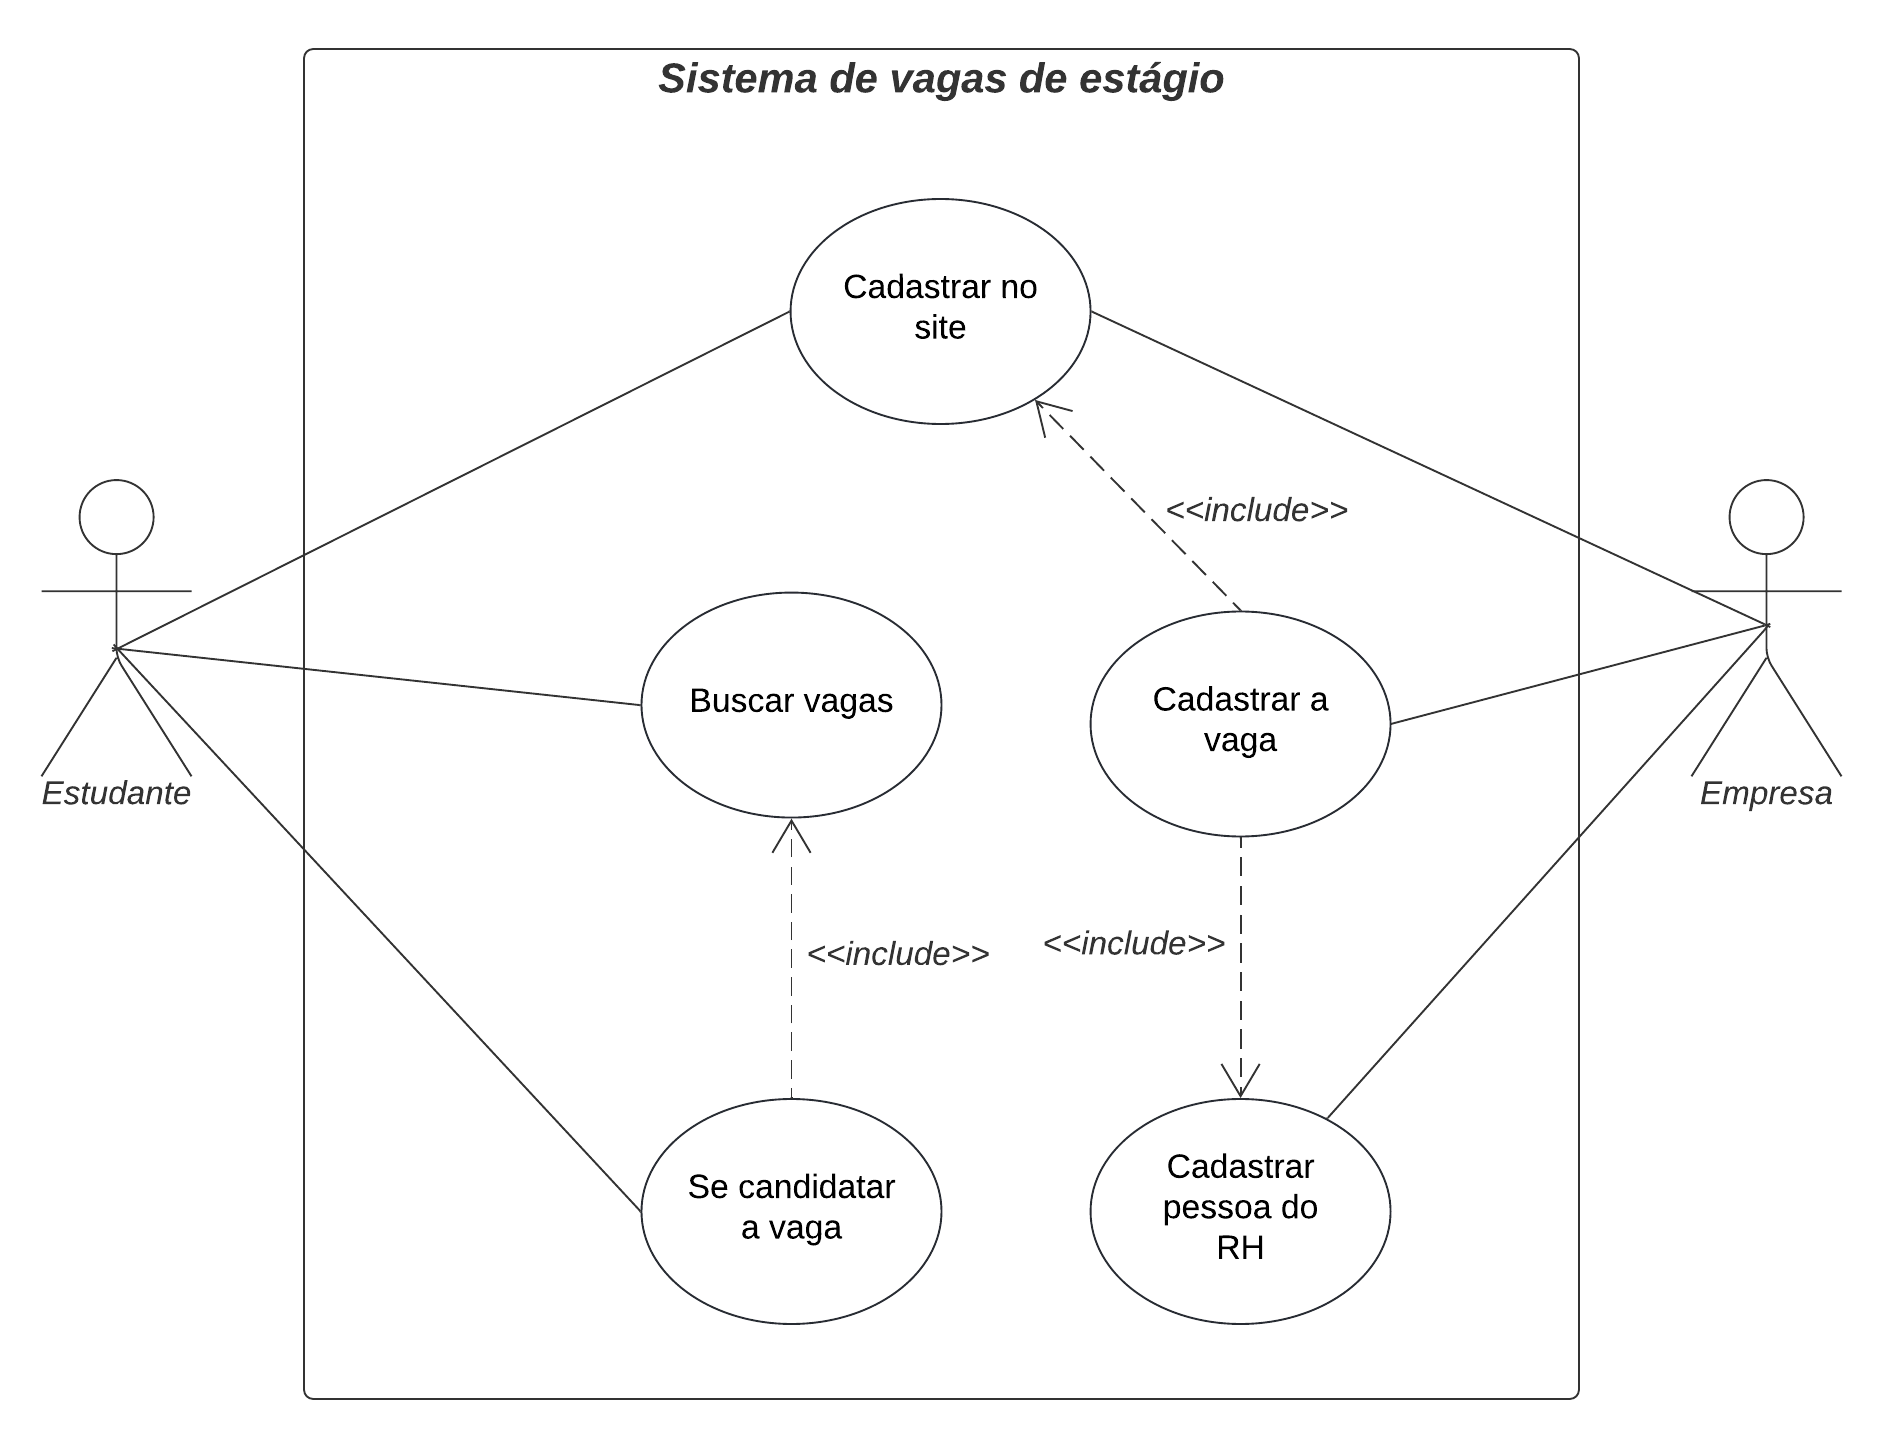
\includegraphics[width=0.8\textwidth]{imagens/caso-de-uso-1.png} 
	\fonte{Os autores}
\end{figure}

\begin{figure}[H]
	\centering 
	\caption{\label{fig:caso2}Caso de Uso 2 - Funcionalidades da empresa}
	%\includesvg[inkscapelatex=false,width=0.6\textwidth]{imagens/caso-de-uso-2.svg}
	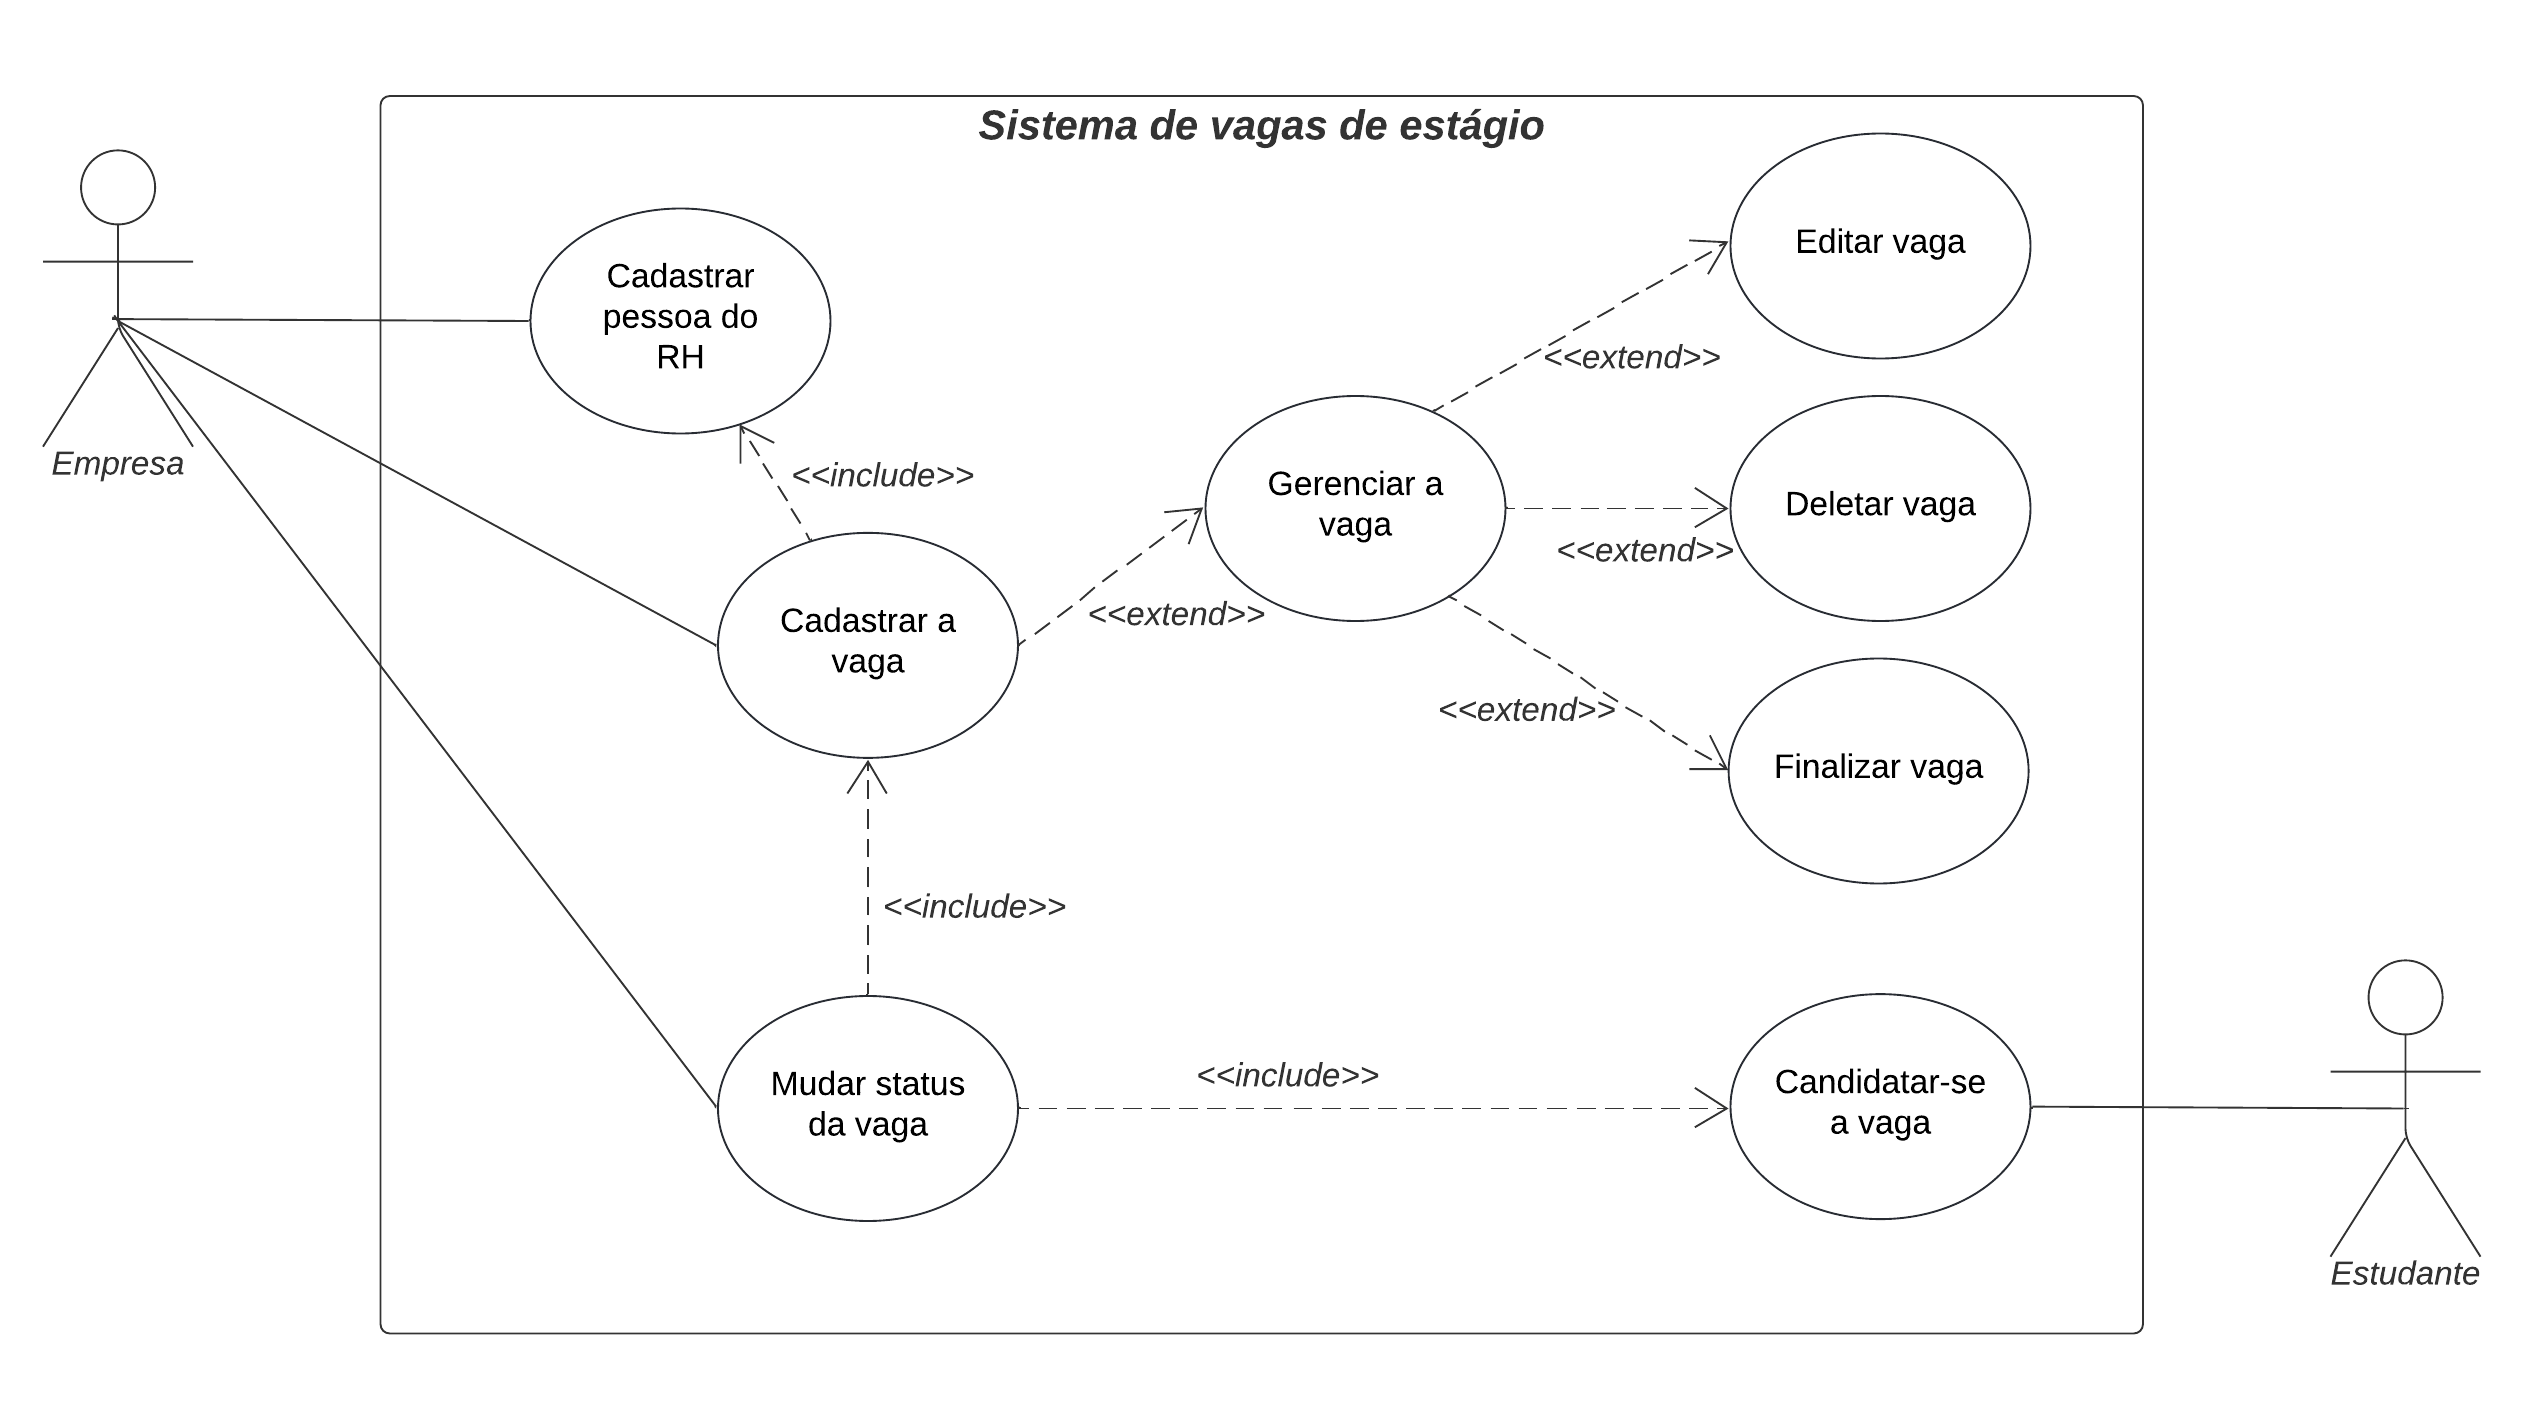
\includegraphics[width=0.8\textwidth]{imagens/caso-de-uso-2.png} 
	\fonte{Os autores}
\end{figure}

\begin{figure}[H]
	\centering 
	\caption{\label{fig:caso3}Caso de Uso 3 - Funcionalidades do administrador}
	%\includesvg[inkscapelatex=false,width=0.6\textwidth]{imagens/caso-de-uso-3.svg}
	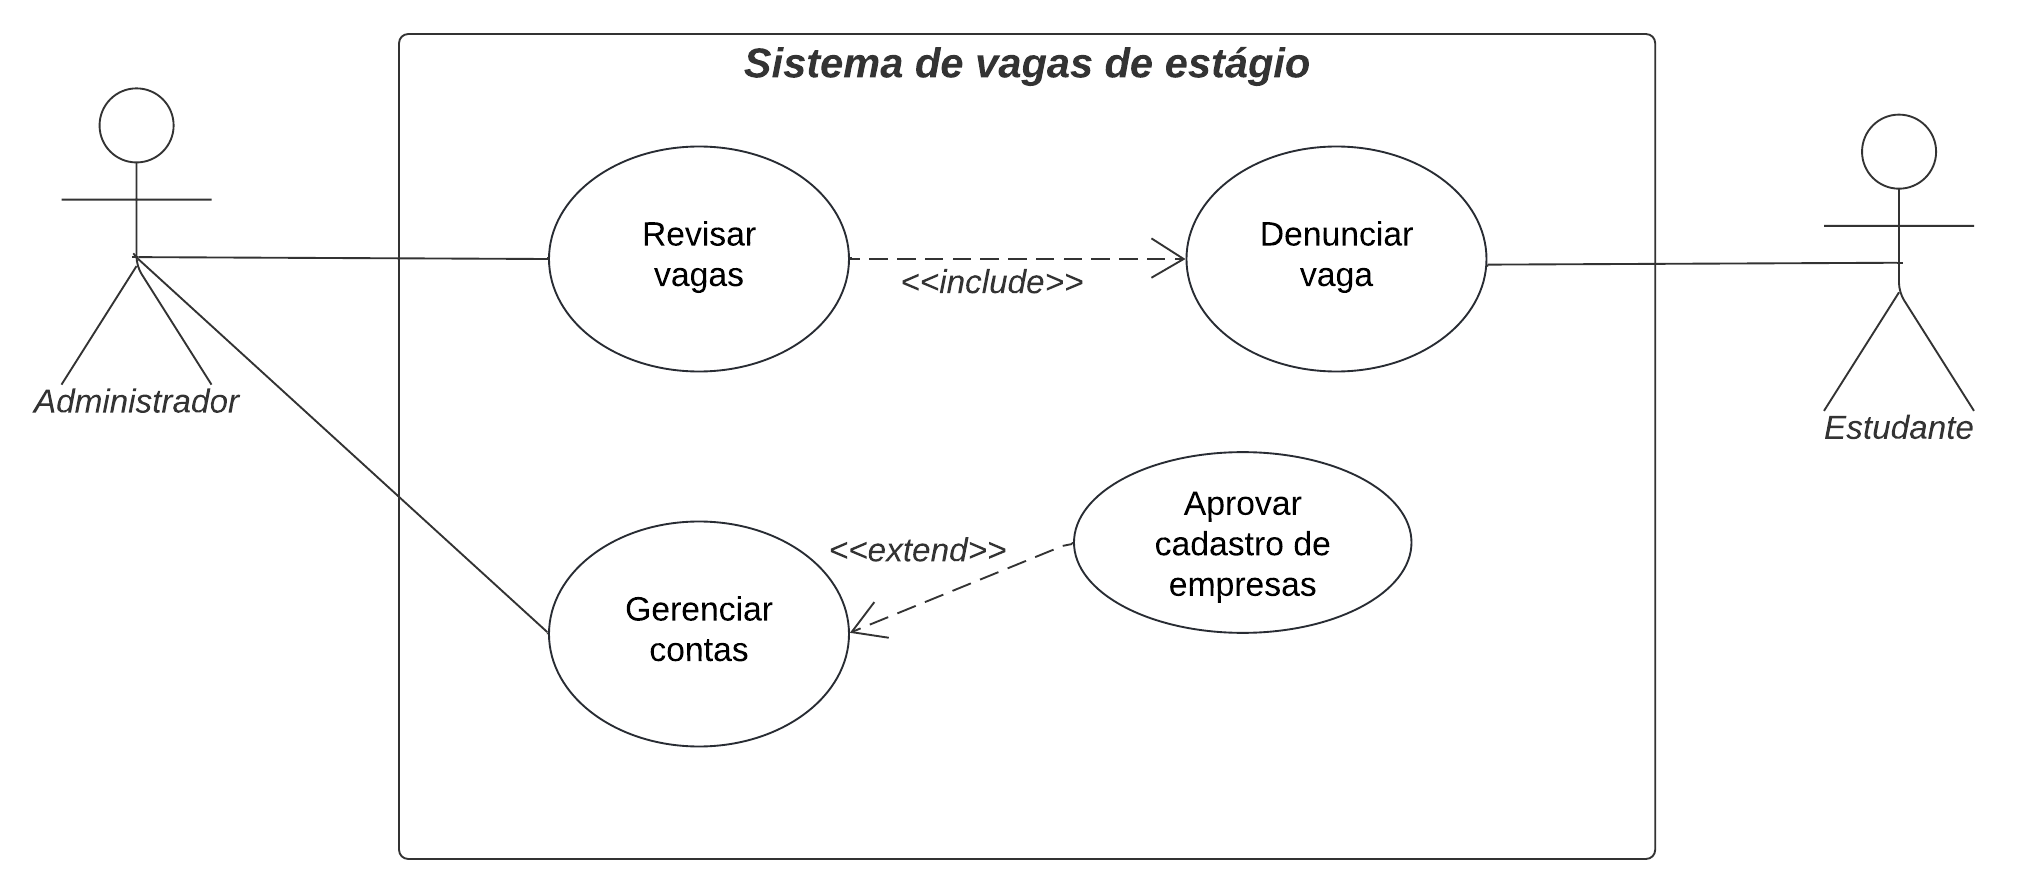
\includegraphics[width=0.8\textwidth]{imagens/caso-de-uso-3.png} 
	\fonte{Os autores}
\end{figure}

\subsection{Fases de entrega}

Nessa seção, iremos expor quais funcionalidades do sistemas pretendemos entregar nas principais fases de entrega.

\subsubsection{Prova de Conceito}

Na fase da prova de conceito, pretendemos entregar as funcionalidades mais básicas do nosso software. Dentre elas, o cadastro de estudantes via \ac{sso} da Google, onde é explicado o processo no site possibilitando a criação de uma conta com informações básicas, necessárias apenas para o funcionamento padrão do sistema, e o cadastro de empresas, que será feito no próprio \emph{website}, onde a empresa preenche as informações e passa por uma aprovação nossa. Além disso, o software permitirá o login desses usuários já cadastrados, onde poderão consultar suas informações básicas.

Ao cadastrar no sistema, a empresa também poderá registrar uma pessoa do \ac{rh} que será responsável por gerenciar as vagas daquela organização, e essa pessoa poderá criar novas vagas com informações básicas, apenas para serem visíveis na tela de consulta de vagas.
Na parte do estudante, será possível para ele, consultar as vagas que existem no sistema através de filtros básicos e internacionalização de linguagem.

\subsubsection{Produto Mínimo Viável (MVP)}

Na entrega do \ac{mvp}, pretendemos incrementar o que já foi desenvolvido durante a prova de conceito com funcionalidades importantes ao nosso sistema, como a candidatura do estudante à uma vaga, a possibilidade do estudante denunciar uma vaga por não ser coerente com a proposta da nossa aplicação, que é ser um \emph{website} que possua vagas de estágios coerentes com a realidade de um estagiário, funcionalidade de login via \gls{linkedin} para os estudantes, recomendações de vagas para os candidatos, recomendação de candidatos para empresas e opção de contato com o candidato via \emph{Whatsapp}. Além disso, serão feitos os teste unitários e testes de qualidade de software, a fim de garantir que a aplicação esteja em conforme com os requisitos solicitados.

\subsubsection{Entrega Final}

Na entrega final, iremos acrescer nosso projeto com o restante das funcionalidades, tais como o \emph{dashboard} de vagas para a empresa, histórico de vagas para os estudantes, mudança de status das vagas por parte da empresa, \emph{feedback} de empresas após o processo seletivo e utilização de mais campos do banco de dados para termos mais detalhes de vagas, usuários, etc.

Além disso, requisitos não funcionais, como a refatoração do código, a fim de deixá-lo mais limpo e performático, e mais testes de qualidade de software, agora com um banco de dados com mais registros, para manter o mesmo nível de performance e usabilidade que tinha antes, com poucos registros.